\chapter{LITERATURE REVIEW}

\section{Vision-Language model}
\subsection{Learning Transferable Visual Models From Natural Language Supervision}
Most computer vision deep learning pre-trained model are trained with specific set of class.
For this reason, most computer vision deep learning models are lack of generalizability and usability.
\shortciteA{clip} proposed pre-training method which utilize image and text description to train vision models called Contrastive Language-Image Pre-training (CLIP).
The overall method is showed in Figure~\ref{fig:clip}.
The training dataset is gather from the internet in a form of (image, text) pairs of 400 million pairs.
The model had a text encoder and an image encoder model.
In \shortcite{clip}, the image encoder models are ResNet and Vision Transformer and the text encoder model are transformer model.
The model is optimized to maximize the similarity between each image text pair with non original image text pair as a negative target for contrastive training.
As a result the CLIP model has generalizability tested by comparing CLIP zero-shot classification and linear probe on ResNet50 as showed in the Figure~\ref{fig:clip-performance}

\begin{figure}[h]
    \caption{Overall method of contrastive language-image pre-training}
    \label{fig:clip}
    \centering
    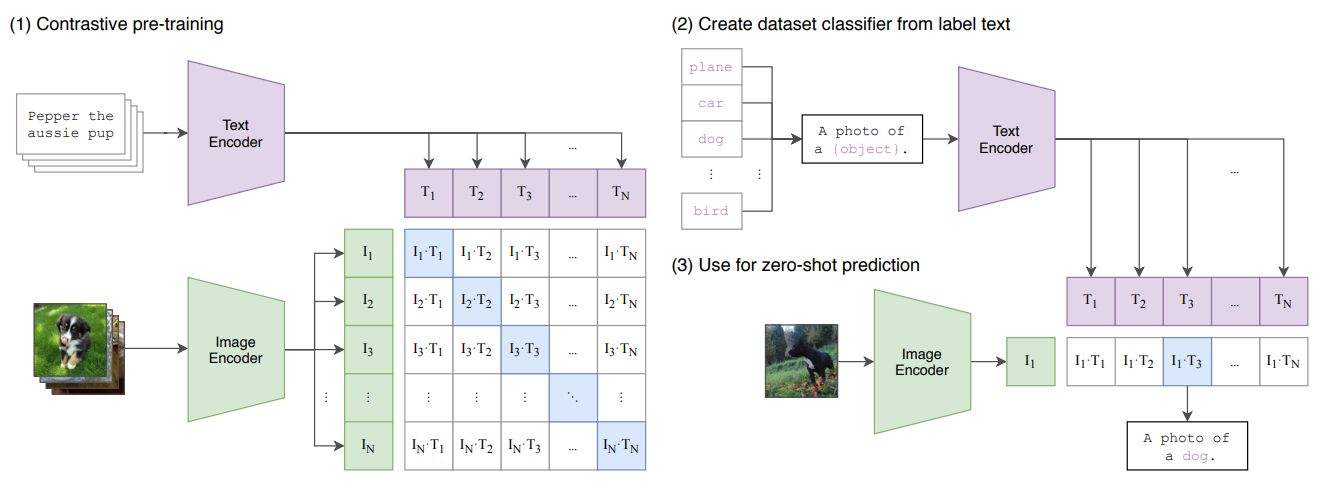
\includegraphics[width=1\textwidth]{Images/CLIP.png}
    \small
\end{figure}

\begin{figure}[h]
    \caption{Zero-shot CLIP is competitive with a fully supervised baseline.}
    \label{fig:clip-performance}
    \centering
    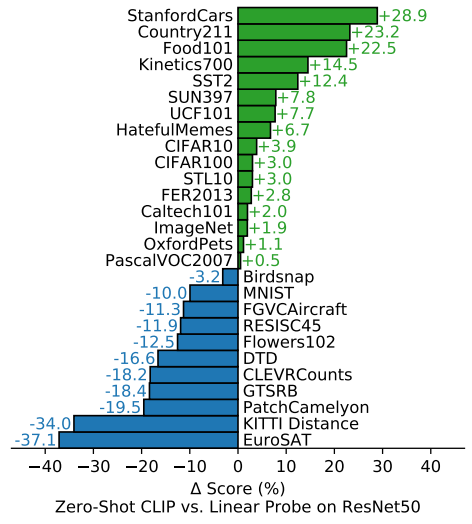
\includegraphics[width=1\textwidth]{Images/CLIPPerformance.png}
    \small
\end{figure}

\subsection{CoCa}


\subsection{mPlug}

\section{Knowledge Distillation and Self-Distillation}
Knowledge Distillation was firstly proposed by \shortciteA{knowledge_distill} to compress the model size while maintaining the model performance as much as possible.
The method contained a smaller student model and a single or multiple larger teacher model.
The knowledge was transferred by optimizing the student model output to match the teacher's output.
\shortciteA{born_again} investigated knowledge distillation using a student model size the same as the teacher model, showing improvement in the student model.
Such a method is called self-distillation.
The self-distillation has widely adopted in semi-supervised image classification tasks, such as Mean Teacher \shortcite{mean_teacher}, EMAN \shortcite{eman} and FixMatch \shortcite{fixmatch}.
DINO \shortciteA{dino} proposed self-distillation pre-training without using any label, which resulted in performance improvement.
In this paper, we extended the self-distillation by creating representation which was image-text combined representation, and we trained the student model to match teacher softmax outputs.

% \section{Semi-Supervised Learning}
% In semi-supervised learning, recent method can be divided into two category, pseudo-labeling and consistency-based. The consistency-based \shortcite{laine2016temporal, tarvainen2017mean, xie2020unsupervised, verma2022interpolation} is focus on training two models by giving same image with difference augmentation, and those two model are train to output very similar probability output using consistency loss. $\Pi$-Model and Temporal Ensemble \shortcite{laine2016temporal} training with consistency loss and adding noise to model weights using dropout. UDA \shortcite{xie2020unsupervised} apply weak and strong image augmentation to train two models simultaneously. On the other  hand, pseudo-labeling \shortcite{sohn2020fixmatch, cai2022semisupervised, pham2021meta} focus on assign label to the unlabeled images by pre-train a teacher model with labeled images. This work is fall into consistency-based group, training with the logits output of the teacher model directly.

% \section{Image Captioning}


% \begin{table}[]
% \begin{tabular}{lllllll}
% Model & Param & Key Contribution                                                            & ImageNet1\%  Top1\% & ImageNet10\% Top1\% &   &   \\
% Semi-ViT/Base 2022 & 86M       & Using Teacher-Student and propose Batch MixUp to mix label and unlabel image & 71.0                & 79.7                &   &   \\
% Semi-ViT/Large     & 307M      &                                                                              & 77.3                & 83.3                &   &   \\
% FixMatch 2020      & ResNet-50 & Propose strong and weak augmentation using consistency regularization        &                     & 71.46               &   &   \\
%                    &           &                                                                              &                     &                     &   &
% \end{tabular}
% \end{table}